In 1915, Albert Einstein published his General Theory of Relativity, a 
geometric theory of gravitation that sought to expand upon Newtonian 
mechanics and provide a complete description of gravity and its 
relationship with space and time. Einstein theorized that space 
and time were deeply related and existed together as a manifold 
called spacetime. Matter with energy and momentum 
existing in this manifold create 
curvature in spacetime. Gravitational forces are the result of 
matter following geodesic curves in spacetime. This concept can 
be summarized in the Einstein field equation, 
\begin{equation}
G_{\mu\nu} = 8\pi T_{\mu\nu}
\label{eq:EFE}
\end{equation}
where $G_{\mu\nu}$ is the Einstein tensor, which describes the 
curvature of spacetime, $T_{\mu\nu}$ is the 
stress-energy tensor, which describes the energy and momentum in 
spacetime, and  $G=c=1$. The Einstein tensor is defined as,
\begin{equation}
G_{\mu\nu} = R_{\mu\nu} - \frac{1}{2}Rg_{\mu\nu}
\end{equation}
where $R_{\mu\nu}$ is the Ricci curvature tensor and $g_{\mu\nu}$ is 
the metric tensor for the manifold.

An interesting result that arises in this theory  is the 
existence of gravitational waves \cite{Einstein:1916,Einstein:1918}, 
which are perturbations in 
spacetime caused by certain types of time-varying mass distributions. 
To describe gravitational waves, we consider 
a Minkowski metric with a small perturbation. The Minkowski metric 
is a flat spacetime metric defined as
\begin{equation}
\eta_{\mu\nu} = 
  \begin{pmatrix}
   -1 & 0 & 0 & 0 \\
    0 & 1 & 0 & 0 \\
    0 & 0 & 1 & 0 \\
    0 & 0 & 0 & 1
  \end{pmatrix}
\end{equation}
where $\mu = 0$ corresponds to the time coordinate and $\mu = {1,2,3}$ 
correspond to the spatial coordinates. In examples, we will use the coordinate 
convention $(x^0,x^1,x^2,x^3) = (ct,x,y,z)$. 
The full spacetime metric, $g_{\mu\nu}$, is then constructed as a 
linear perturbation on the Minkowski metric,
\begin{equation}
g_{\mu\nu} = \eta_{\mu\nu} + h_{\mu\nu}
\end{equation}
where $h_{\mu\nu}$ is the metric perturbation and $|h_{\mu\nu}| \ll 1$.

To explore the effects of this perturbation, it is very useful to move 
into the transverse traceless 
gauge where coordinates on the manifold are defined by the geodesic 
motion of freely-falling test masses \cite{Saulson:1994}. In this gauge, the weak field 
vacuum solution of the Einstein field equation becomes a wave equation: 
\begin{equation}
\square h_{\mu\nu} = 0.
\end{equation}
The solutions to this differential equation will be plane waves of 
the form
\begin{equation}
h_{\mu\nu} = C_{\mu\nu}e^{i(2\pi ft - \vec{k}\cdot\vec{x})}
\end{equation}
where $C_{\mu\nu}$ is the wave amplitude, $f$ is the frequency, 
and $\vec{k}$ is the wave vector which indicates the direction of 
propagation \cite{Carroll}.

For example, consider the case of a gravitational 
wave propagating along the $\hat{z}$-axis.
When the conditions of the transverse traceless gauge are applied, 
the resulting form of $h_{\mu\nu}$ is 
\begin{equation}
h_{\mu\nu} = 
  \begin{pmatrix}
    0 & 0 & 0 & 0 \\
    0 & h_+ & h_\times & 0 \\
    0 & h_\times & -h_+ & 0 \\
    0 & 0 & 0 & 0
  \end{pmatrix}
\label{eq:strain}
\end{equation}
where the diagonal and off-diagonal terms represent two polarizations 
of the resulting gravitational wave, called ``h-plus" and ``h-cross" 
respectively.
We can see the effects of this perturbation by observing the  
spacetime interval on the manifold. The spacetime interval is defined as 
\begin{equation}
ds^2 = dx^\mu g_{\mu\nu}dx^\nu.
\end{equation}
Substituting in our perturbed metric for $g_{\mu\nu}$, we find that 
the spacetime interval can be broken up into a standard Minkowski line 
element and a perturbation due to $h_{\mu\nu}$.
\begin{equation}
ds^2 = dx^\mu (\eta_{\mu\nu} + h_{\mu\nu})dx^\nu \\
\end{equation}
\begin{equation}
ds^2 = dx^\mu \eta_{\mu\nu} dx^\nu + dx^\mu h_{\mu\nu}dx^\nu
\label{eq:spacetime}
\end{equation}

As an example, we present the case of a plus-polarized gravitational wave 
propagating in the $\hat{z}$ direction and observe the effect of the perturbation 
on the spacetime interval. The perturbation will have the form 
\begin{equation}
h_{\mu\nu} = 
  \begin{pmatrix}
    0 & 0 & 0 & 0 \\
    0 & h_+ & 0 & 0 \\
    0 & 0 & -h_+ & 0 \\
    0 & 0 & 0 & 0
  \end{pmatrix}
\end{equation}
Using the coordinate convention of $(ct,x,y,z)$, the unperturbed
spacetime interval is given as: 
\begin{equation}
ds^2 = -c^2 dt^2 + dx^2 + dy^2 + dz^2.
\end{equation}
Since the perturbation is spatially transverse to the direction of 
propagation, the ct- and $\hat{z}$-coordinates will not be modulated by the 
gravitational wave. The $\hat{x}$- and $\hat{y}$-coordinates will be modulated  
according to equation \ref{eq:spacetime}. The resulting spacetime 
interval is
\begin{equation}
ds^2 = -c^2 dt^2 + (1 + h_+)dx^2 + (1 - h_+)dy^2 + dz^2.
\end{equation}
This shows that a gravitational wave propagating along the $\hat{z}$-axis 
will differentially stretch and squeeze spacetime in the transverse 
axes. The exact form of $h_+$ will depend on the source of the 
gravitational waves. A visualization of this stretching and squeezing 
is shown in Figure \ref{fig:polarizations} \cite{Polarization}. The cross polarization  
stretches and squeezes at a 45 degree angle relative to the plus 
polarization. The strain, $h$, imparted by a gravitational wave is 
typically extremely small by the time it reaches Earth, producing 
relative length changes on the order of $10^{-22}$. 

\begin{figure}[ht!]
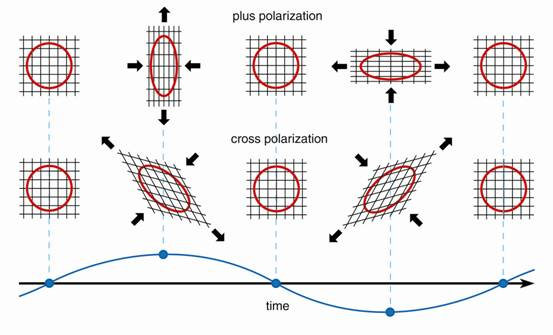
\includegraphics[width=\textwidth]{figures/introduction/polarisations2}
\caption[Plus and cross polarizations]{Plus and cross polarizations %
         of a gravitational wave. As a gravitational wave propagates through spacetime, %
         there is a stretching and squeezing effect that changes the relative length between %
         points in spacetime. The strain produced by the cross polarization %
         is at a 45 degree angle relative to the strain produced by the plus %
         polarization. }
\label{fig:polarizations}
\end{figure}

The Advanced LIGO interferometers are designed to be sensitive 
to this differential stretching and squeezing by constructing orthogonal 
optical cavities, referred to as the X- and Y-arms. 
When a gravitational wave passes through a LIGO inteferometer, the length of 
the arms is modulated, causing the light to have a
longer or shorter travel time as it traverses the optical cavities. 
Since gravitational
waves expand space in one direction while the orthogonal direction contracts,     
the X- and Y-arms will experience differential changes in length. When light
from the arms is recombined, there will be a difference
in phase between the two beams as they have traveled different paths. 
The result of this phase mismatch is a change in optical power at the output 
port of the interferometer. This output optical signal can be searched for 
evidence of interactions with gravitational waves.
The layout and gravitational wave readout scheme of the interferometers is 
discussed below.

\section{The Advanced LIGO Interferometers}\label{sec:aligo}

The Advanced LIGO (aLIGO) interferometers are a pair of dual-recycled Michelson interferometers 
that employ 4km long Fabry-Perot cavities in their arms to increase the interaction time with a 
gravitational wave signal. 
Figure \ref{fig:aligo} shows a simplified layout of an aLIGO interferometer. 

\begin{figure}[ht!]
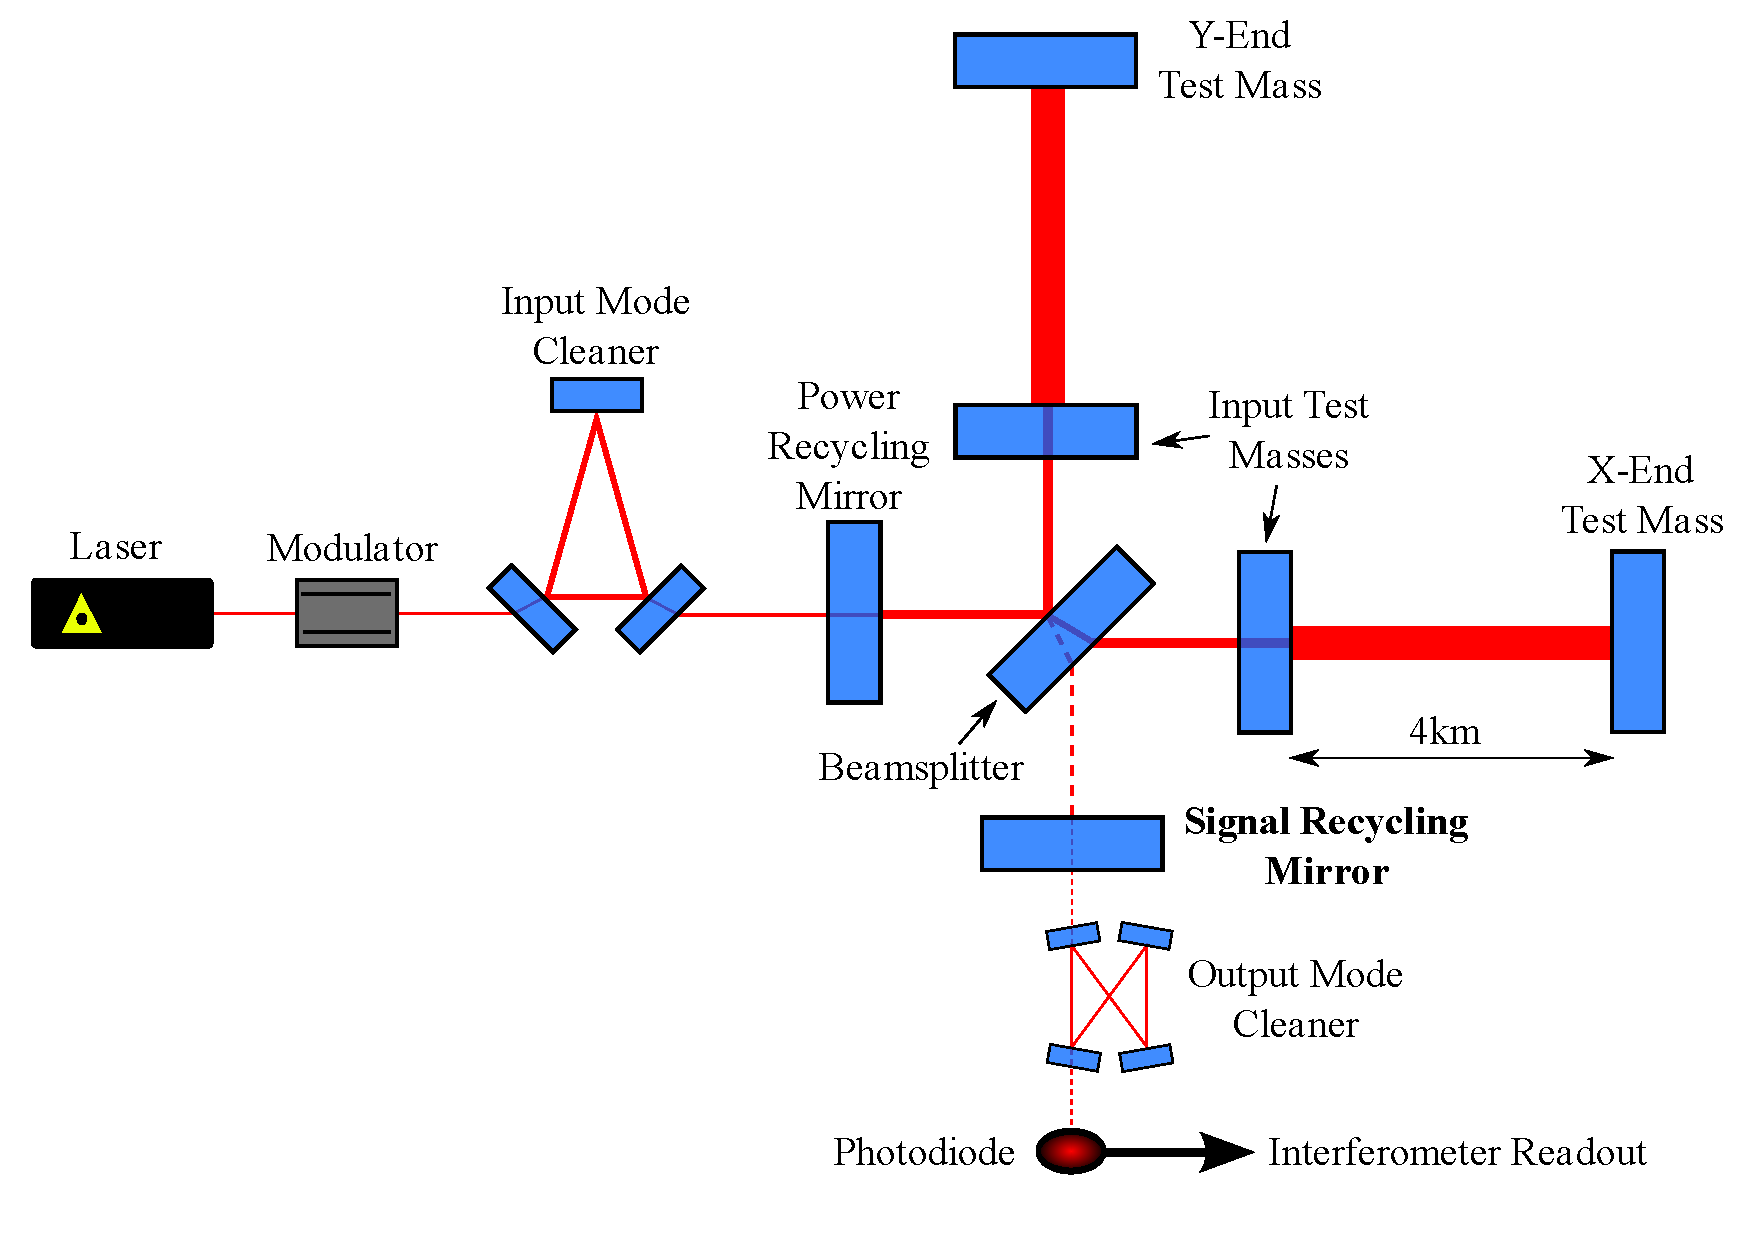
\includegraphics[width=\textwidth]{figures/introduction/ALIGO_layout}
\caption[Layout of Advanced LIGO]{Layout of Advanced LIGO}
\label{fig:aligo}
\end{figure}

At the input to an aLIGO interferometer is a solid-state Nd:YAG laser that provides laser light 
at a wavelength of 1064 nm. Not included in Figure \ref{fig:aligo} are frequency and 
intensity stabilization control loops designed to provide as stable a laser source as 
possible for the experiment. This stabilized laser is called the pre-stabilized laser 
(PSL). The laser light is passed through a series of 
electro-optic modulators (EOM) where radio-frequency (RF) sidebands are generated 
and imparted onto the light. These RF sidebands are used to sense auxiliary optical 
degrees of freedom in the interferometer. The beam is then passed through the 
input mode cleaner (IMC), which rejects higher order spatial modes of the beam 
and transmits a circular TEM00 mode to be used in the instrument.

Once the beam has been stabilized in frequency and intensity and the higher order 
optical modes have been stripped away, it is transmitted through the power 
recycling mirror and enters the vertex of the interferometer. In the vertex, 
the beam is split 50/50 by the beamsplitter. Half of the light is directed toward  
the input test mass (ITM) of the X-arm and half of the light is directed  
toward the ITM of the Y-arm. As mentioned previously, the aLIGO arms are not 
single bounce cavities; they are comprised of Fabry-Perot cavities that allow the 
light to circulate in the arm cavities multiple times. The light is stored in 
the arm cavities for $\sim$1ms, trapped between the highly reflective surfaces 
of the ITM and the end test mass (ETM), before it is transmitted back through 
the ITM and into the vertex.

As mentioned above, it is the interaction of the arm cavities with gravitational 
waves that allows the optical field to be imparted with a gravitational wave signal. 
The increased light storage time provided by Fabry-Perot cavities increases the 
interaction between the optical field and a gravitational wave by increasing 
the effective optical length of the arm cavities. 
An incident gravitational wave differentially modulates the arm cavities, resulting 
in a difference in path length for the beams traveling in each arm.  

When light
from the arms is recombined at the beamsplitter, there will be a difference
in phase between the two beams if they have traveled different paths. The 
resulting light from this recombination of phase shifted beams will 
be divided based on how much of a phase offset was accumulated as the 
beams traversed the arms. In the absence of a gravitational wave, most of the 
light will be directed back toward the power recycling mirror. This is called 
the symmetric port of the interferometer. A small amount of light is directed 
toward the signal recycling cavity. This is called the antisymmetric port of 
the interferometer. The optical power at these ports will fluctuate in the 
presence of a gravitational wave. It is the antisymmetric port optical field 
that is used to search for gravitational wave signals.

At the symmetric port, the beam 
will be sent back toward the power recycling mirror. The power recycling mirror 
forms a resonant cavity with the ITMs, allowing for light at the symmetric 
port of the beamsplitter to be added coherently to incoming light from the PSL and 
increasing the effective power in the vertex. This increase in effective power 
is known as the power recycling gain. 

At the antisymmetric port, the beam is sent toward the signal recycling mirror. 
The signal recycling cavity is used to increase the sensitivity of the 
interferometer in a band of frequencies by adjusting the effective finesse 
of the coupled cavity 
formed by the signal recycling cavity and the arm cavities. 
If the light returning from the arms has accumulated some differential amount of 
phase as it traveled 
along the arms, perhaps from a gravitational wave modulating the length of each 
arm differentially, it will be transmitted through the signal recycling cavity 
and into the output mode cleaner (OMC). The OMC behaves similarly to the IMC, 
stripping away higher order optical modes and isolating the TEM00 mode of the 
beam. The transmitted, mode cleaned signal is then read out using a homodyne 
detection scheme on a DC photodiode.

\subsection{DC Readout}

When a gravitational wave modulates the length of an arm cavity, the light 
traveling in that arm experiences a phase modulation. This phase modulation 
can be visualized by picturing the beam in frequency space. In Figure 
\ref{fig:omc-freq}, the carrier beam frequency is designated as $f_0$. 
The phase modulation due to 
a gravitational wave signal introduces a frequency sideband at the 
gravitational wave frequency, which is in the kHz range for signals that 
LIGO is sensitive to. 
The 
RF sidebands used for auxiliary optical cavity control are offset from the 
carrier frequency by 9, 24, and 45 MHz. 
In a heterodyne detection scheme, the interferometer would operate at the 
'dark fringe', meaning that the output port would not transmit light until 
there was differential arm motion. In this scheme, the RF sidebands would be 
detected on the same photodetector as the gravitational wave sidebands. The 
RF sidebands would be used to demodulate the photodetector signal, leaving 
behind a gravitational wave signal. This is the method that was used in 
initial LIGO.

In Advanced LIGO, a homodyne detection, or 'DC Readout', scheme is employed 
\cite{DCReadout}. 
In a homodyne detection scheme, the RF sidebands are not used to extract the 
gravitational wave signal. Instead, the carrier beam itself is used. Instead of 
aligning the instrument on the dark fringe, an differential offset is introduced 
to the arm cavities to allow a small amount of light into the output port. 
The RF sidebands, which if not used for demodulation would only contribute 
noise to the output signal, 
are rejected by the output mode cleaner (OMC). 
The gravitational wave sidebands, however, are at a 
low enough frequency offset that they are within the pass band of the OMC 
and are allowed to transmit through the cavity.

Since the OMC DC photodiode measures power, it measures the square of the 
incident optical field and witnesses beat frequencies between different 
components of the light. If the RF sidebands have been filtered out by 
the OMC, the only remaining beat note will be that of the carrier beam ($f_0$) 
beating against the gravitational wave sideband ($f_0 + f_{GW}$). This beat note will 
appear as the difference in frequency between the two optical fields, 
leaving behind a signal in the 30-2000 Hz range ($f_{GW}$) and providing a 
natural demodulation inherent to the measurement process. 
The process of recovering the gravitational wave sideband using the 
carrier field as a reference is known as homodyne detection. The 
advantage in this method lies in the fact that the carrier beam 
has been passed through the arm cavities. The cavities act as a low 
pass filter and remove high frequency noise relative to the carrier 
beam frequency. The RF sidebands are quite noisy in comparison and this 
noise is propagated forward when they are used for demodulation. 

\begin{figure}[ht!]
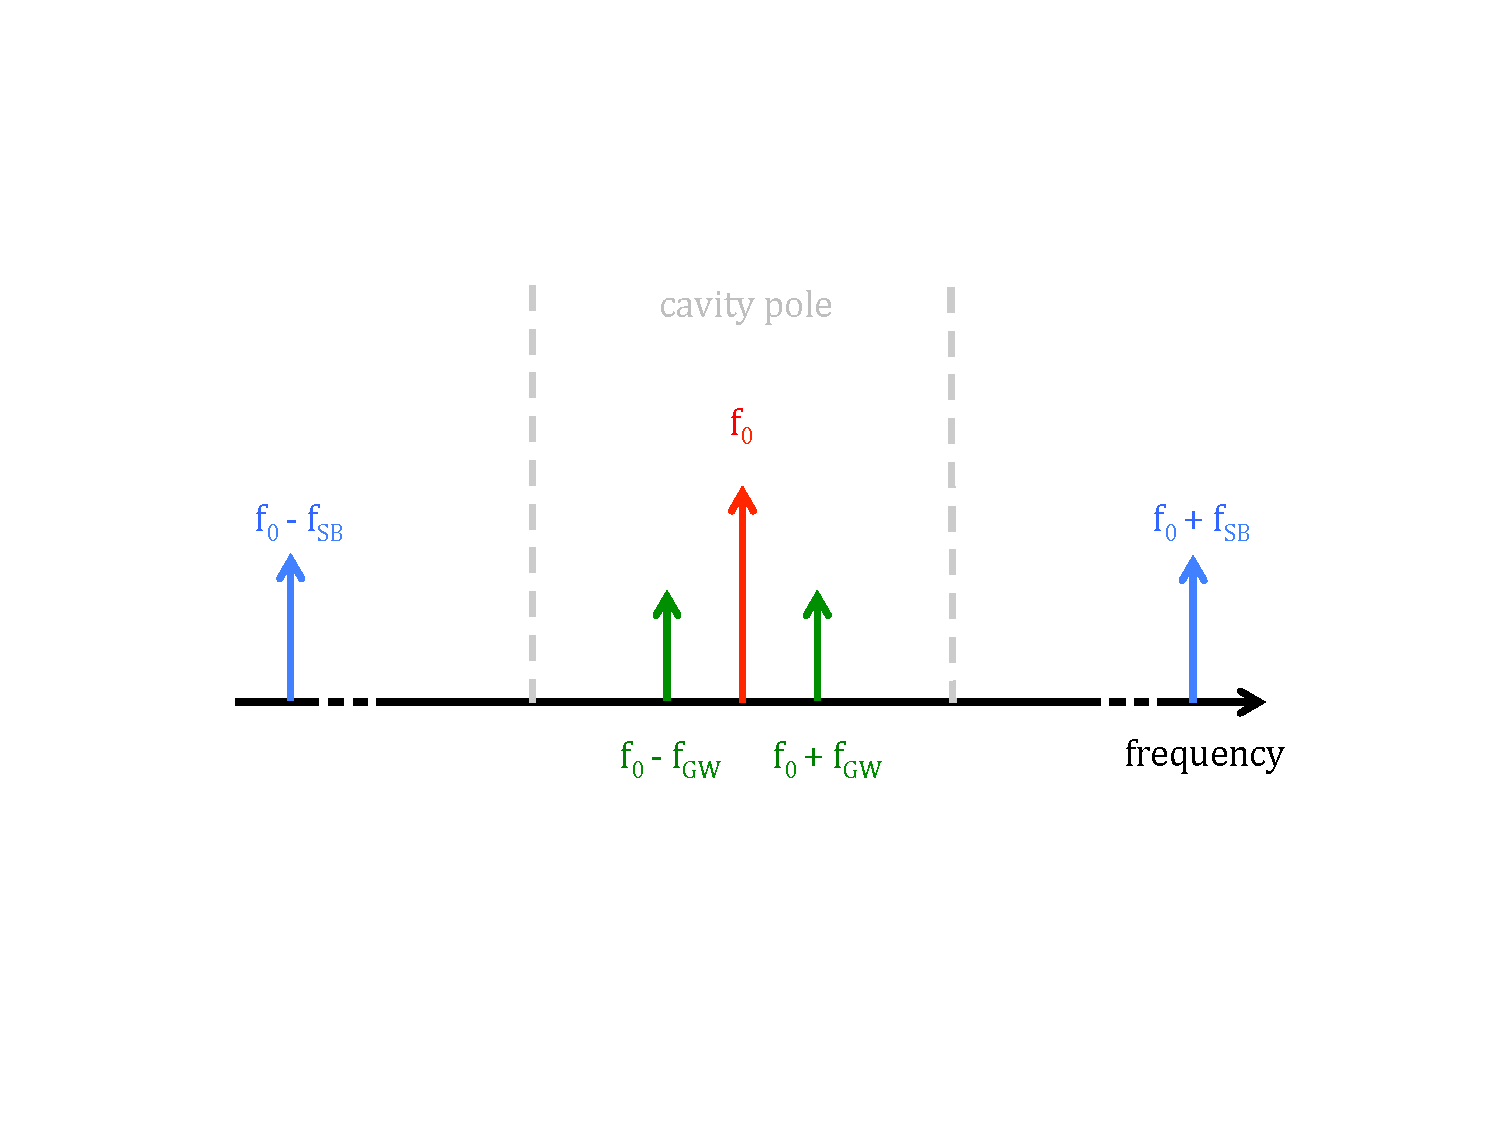
\includegraphics[width=\textwidth]{figures/introduction/omc-freq}
\caption[Sidebands and OMC cavity pole]{Frequency domain visualization of beam %
         at OMC. Grey dotted lines indicate the cavity pole. The gravitational %
         wave sidebands are within the cavity pole and are transmitted through %
         the OMC. The RF sidebands are in the MHz range and are rejected by the %
         OMC.}
\label{fig:omc-freq}
\end{figure}


\subsection{The aLIGO Noise Curve}

The aLIGO interferometers are among the most precise measuring devices 
that have ever been constructed, sensitive to a differential displacement 
on the order of $10^{-19}$ m$/\sqrt{Hz}$ at their most sensitive frequencies. 
When operating at such small length scales, 
the interferometers are susceptible to a number of very subtle noise sources. 
Figure \ref{fig:noise-budget} shows the limiting noise sources for the 
aLIGO interferometers \cite{GW150914-DETECTORS}. Each curve represents 
a known source of noise in the interferometer output. 

\begin{figure}[ht!]
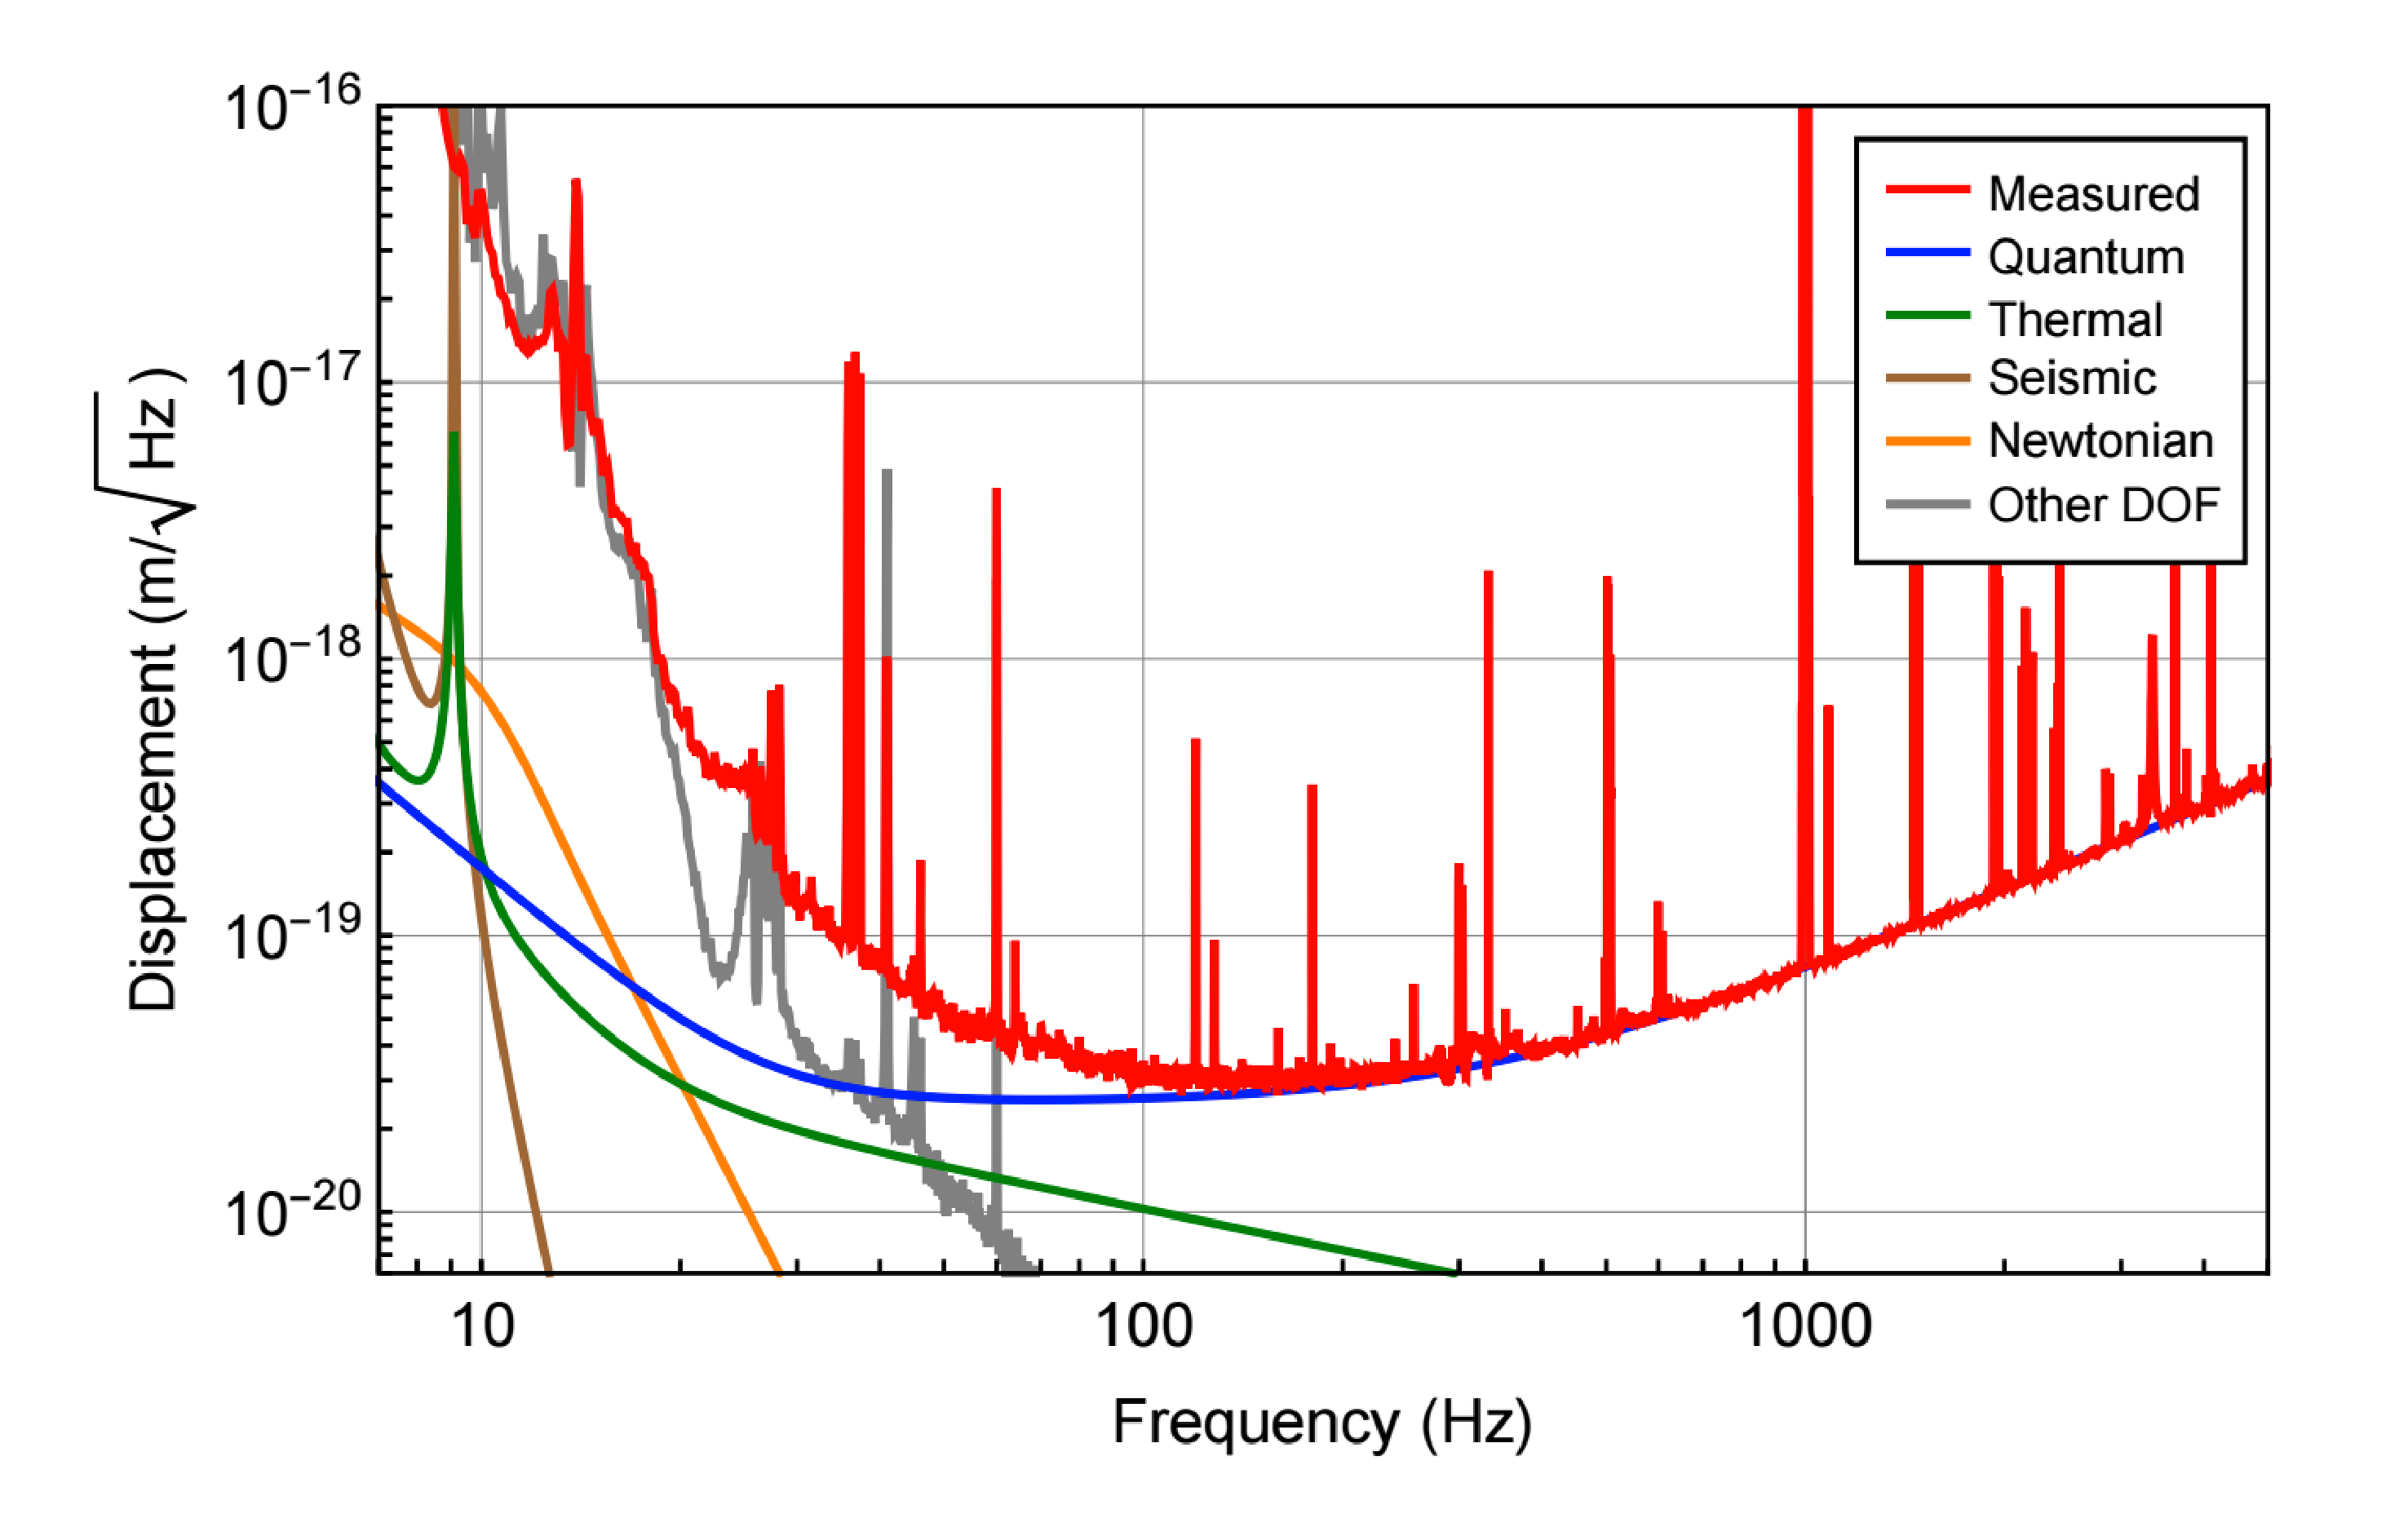
\includegraphics[width=\textwidth]{figures/introduction/noise-budget}
\caption[Advanced LIGO noise budget]{Advanced LIGO noise curve during the first %
         observing run with %
         understood noise sources, reproduced from \cite{GW150914-DETECTORS}. %
         The red curve is the measured instrumental noise at Hanford during the first %
         observing run. The blue curve is quantum noise, which is a combination of %
         photon shot noise at the output photodetector and radiation pressure noise %
         on the test mass optics. The green curve is the modeled thermal noise, which is a %
         combination of thermal noise from the suspensions, optics, and optical %
         coatings. The brown curve is seismic noise coupling into the optics, %
         which is highly attenuated at high frequencies. The orange curve is %
         Newtonian noise, which is driven by perturbations in the density of %
         the ground. The grey curve labeled 'Other DOF' is the sum of the %
         noise coupling from auxiliary optics into the output of the interferometer, %
         mainly driven by optical misalignments.
        }
\label{fig:noise-budget}
\end{figure}

At frequencies below 10 Hz, the limiting noise at design sensitivity 
comes a combination of seismic 
noise and suspension thermal noise. Seismic noise is caused by vibrations coupling 
from the Earth onto the mechanical structures supporting the aLIGO optics. 
Seismic noise is attenuated using 
a multi-tiered active feedback seismic isolation system \cite{SeiReview,HEPI}. At higher 
frequencies, any residual seismic noise is passively attenuated by the 
suspension systems, which use multiple stages of pendula to reduce displacement noise 
from the suspension point to the optics.
Suspension thermal noise is dominated by the mechanical losses of the fused 
silica fibers used to suspend the test masses. 
Since the interferometers have not yet been fully commissioned, the current 
limiting noise below 10 Hz is driven by noise coupling from auxiliary 
degrees of freedom.

From 30 Hz onwards, there will eventually be two dominant noise sources: quantum noise 
(the blue curve in Figure \ref{fig:noise-budget}) 
and coating Brownian noise (the green curve in Figure \ref{fig:noise-budget}). 
Quantum noise is the combination of two sources. 
The first is shot noise, which is a photon counting noise when light is measured 
on a photodiode. Shot noise is the dominant noise source above $\sim$300 Hz and 
can be further improved by increasing laser power. 
The second is radiation pressure noise, which is a fluctuating 
force on the test masses based on fluctuations in photon number in the cavity. 
Radiation pressure noise will increase with increasing laser power as 
a higher photon number implies a higher uncertainty in the momentum 
imparted onto the test mass optics.
Coating Brownian noise is due to thermally driven mechanical losses in optical 
coatings. 
Figure \ref{fig:noise-budget} shows that the interferometer noise is 
limited by the combination of thermal noise and quantum noise from 100 Hz 
onward. 

\section{Sources of Gravitational Waves}

Gravitational wave signals have highly 
varying characteristics depending on the source of the gravitational 
waves. The gravitational wave strain produced depends on the distribution 
of mass-energy at the source and is given as
\begin{equation}
h_{ij} = \frac{2}{r}\ddot{I}_{ij}
\end{equation}
where $\ddot{I}_{ij}$ is the quadropole tensor describing the 
mass-energy distribution and $c=G=1$. This equation tells us that 
a source distribution requires an accelerating quadropole moment to 
generate gravitational waves. Depending on the dynamics of the source 
system, the resulting gravitational wave signals will vary greatly in 
both duration and morphology.

There are a number of potential sources of gravitational waves that are 
searched for in aLIGO data. Astrophysical searches include both modeled and unmodeled 
searches for both transient and continuous signals. Table \ref{tab:sources} 
gives an example of each of these sources. Each of these categories are 
discussed in the following sections.

\begin{table}[!ht]%
  \begin{tabular}{|c|c|c|}
  \hline
    & Transient  & Continuous  \\
  \hline
  Modeled & Compact binary coalescences & Rotating neutron stars  \\
  \hline
  Unmodeled & Core-collapse supernovae & Stochastic GW background \\
  \hline
  \end{tabular}
  \caption[Table of GW sources]{Table describing sources of %
           gravitational waves.}
  \label{tab:sources}
\end{table}

\subsection{Compact binary coalescences}

Compact binary coalescences (CBC) are a primary search target of the 
Advanced LIGO interferometers. These signals are the result of two 
compact objects, such as neutron stars or black holes, in a binary 
system. The two objects will lose energy as they orbit around each other 
and deform spacetime, generating gravitational waves. As the binary 
system loses energy, the orbit decays until they merge and coalesce 
into one final 
compact object. The orbital frequency of such systems increases 
monotonically as the orbit decays, resulting in a gravitational 
wave signal that sweeps upwards in frequency known as a 'chirp'. 
Since the gravitational wave signal from such a system is known, 
this model is incorporated into the search algorithm and the 
search is referred to as a modeled search. CBC waveforms will 
have a duration from $\sim$0.1-60s in the frequency range that
aLIGO is sensitive to and as such they are considered transient 
signals. Searches for CBC 
signals are discussed in Section \ref{ch:CBCSearches}.

Of particular interest to aLIGO are binary neutron star systems, 
which are known to exist from astronomical 
observation. The 1993 Nobel Prize in Physics was awared to Hulse and 
Taylor for the indirect detection of gravitational waves from a binary 
neutron star system. The orbital 
period of the Hulse-Taylor binary neutron star system has been measured 
since 1974. The decay of its orbital period matches the 
expected orbital decay based on energy loss due to the emission of 
gravitational waves. 

Beyond binary neutron stars, the search for compact binary coalescences 
is expanded to search for binary black hole (BBH) systems and neutron star-black 
hole (NSBH) systems. The discovery of gravitational waves from binary black holes 
was accomplished in the 
first observing run with the discovery of two binary black hole systems, GW150914 
and GW151226. Further discussion of the results from the first observing run is 
presented in Chapter \ref{ch:o1results}.

\subsection{Burst signals}

A predicted population of signals is from unmodeled gravitational 
wave transients, or 'bursts'. These signals can come from core-collapse 
supernovae, cosmic string cusps, and binary black hole mergers 
\cite{Damour:2004kw,GW150914-BURST,lrr-2011-1}. The Advanced LIGO burst 
search is carried out by a number of search pipelines 
\cite{Lynch:2015,BayesWave,Klimenko:2007hd}. 
In a burst search, there are two primary methods for signal identification. 
In a standard burst search, potential signals are identified on a single detector 
basis using an excess power ranking statistic and then checked for coincidence 
between the two interferometers. In a coherent burst search, the data streams 
from both interferometers are combined into one coherent ranking statistic based 
on a maximum likelihood analysis. Each analysis uses their own methods to 
distinguish potential signals from noise.

\subsection{Continuous waves}

Continuous sources of gravitational waves are those that are constantly emitting 
gravitational waves. The primary expected source of continuous gravitational 
waves are rotating neutron stars that have some asymmetry with respect to their 
axis of rotation. If a neutron star has a mountain on it, its rotation will 
produce a time-changing quadropole moment and constantly generate periodic 
gravitational waves. These waves are not expected to be as loud as the 
gravitational waves generated from more violent, transient events. As such, 
the strategy to discover them is different than that of a transient search.

To search for gravitational waves from continuous sources, the data are 
transformed into the frequency domain and integrated for long periods of 
time \cite{CW-all-sky,EinsteinHome}. 
If there is a constant, periodic gravitational wave signal in the data, it 
will manifest as a peak in the frequency spectrum of the data. This peak will 
accumulate signal and grow over the integration period relative to the 
noise floor. 

\subsection{Stochastic background}

In addition to sources that can be directly detected in the data, there is 
also a search designed to discover a stochastic background of gravitational waves
 \cite{Collaboration:S4Stochastic,GW150914-STOCHASTIC}. 
This stochastic background is the superposition of gravitational wave signals that 
are too weak to be detected directly, such as distant compact binaries and 
supernovae. The stochastic background is a statistical background based on the 
rate and distribution of gravitational wave sources in the universe. To resolve 
the stochastic background, the data from the two interferometers are 
cross-correlated over long periods of time. Since the cross-correlation 
is an integral in the time domain, the effects of quiet, correlated 
gravitational wave signals are accumulated over time until a statistically 
significant signal-to-noise ratio can be quoted \cite{Allen1999Stoch}. 
This is an interesting search from a detector characterization point of view, 
as it requires an understanding of correlated noise sources between the two 
interferometers. 

\section{The Advanced Detector Network}

The Advanced Laser Interferometer Gravitational-Wave Observatory is 
part of a worldwide effort to detect gravitational waves from astrophysical 
sources. The two aLIGO interferometers, one in Hanford, WA and one in 
Livingston, LA, are part of a growing network of ground-based interferometric 
gravitational wave detectors. The aLIGO detectors are currently the largest 
and most sensitive interferometric gravitational wave detectors in the 
network.

There are a number of other interferometric gravitational wave detectors 
being built and commissioned for future use in collaboration with aLIGO.
The Advanced VIRGO detector is being built and commissioned in Cascina, Italy 
and will be joining LIGO in observing runs soon. 
The VIRGO interferometer will provide enough 
sensitivity to aid in detection and triangulation of astrophysical sources.

The GEO600 detector, located in Hanover, Germany is an interferometer built in 
collaboration between Germany and the United Kingdom. 
GEO600 is an extremely valuable test bed for interferometric technologies,
including quantum optics and homodyne detection. However, with 600m arms, GEO600 
is unlikely to be sensitive enough to witness expected astrophysical sources.

The KAGRA detector, located underground in the Kamioka mine in Japan, 
is in its commissioning phase. KAGRA has 3 km long arms and, 
unlike other gravitational wave interferometers, employs cryogenics to 
reduce thermal noise in its optics. When complete, KAGRA should be 
sensitive enough to contribute to the worldwide detector network.

A third LIGO interferometer, IndIGO, is in the planning stages and will be 
constructed in India. The position and sensitivty of IndIGO will allow for 
confident triangulation of astrophysical sources of gravitational waves.
